\documentclass[margin=5pt]{standalone}

\usepackage{tikz}
\usetikzlibrary{positioning,automata, matrix, trees, fit}
\usetikzlibrary{calc,backgrounds}
\usetikzlibrary{arrows, arrows.meta}
\usepackage[default]{opensans}

\tikzset{myarrow/.style={-{Stealth[length=3mm, width=2mm, sep=1pt]}}} 
\tikzset{mybackarrow/.style={{Stealth[length=3mm, width=2mm, sep=1pt]}-}} 
\tikzset{beschriftung/.style={font=\fontsize{15}{0}\selectfont}} 

\begin{document}
%	\sffamily

	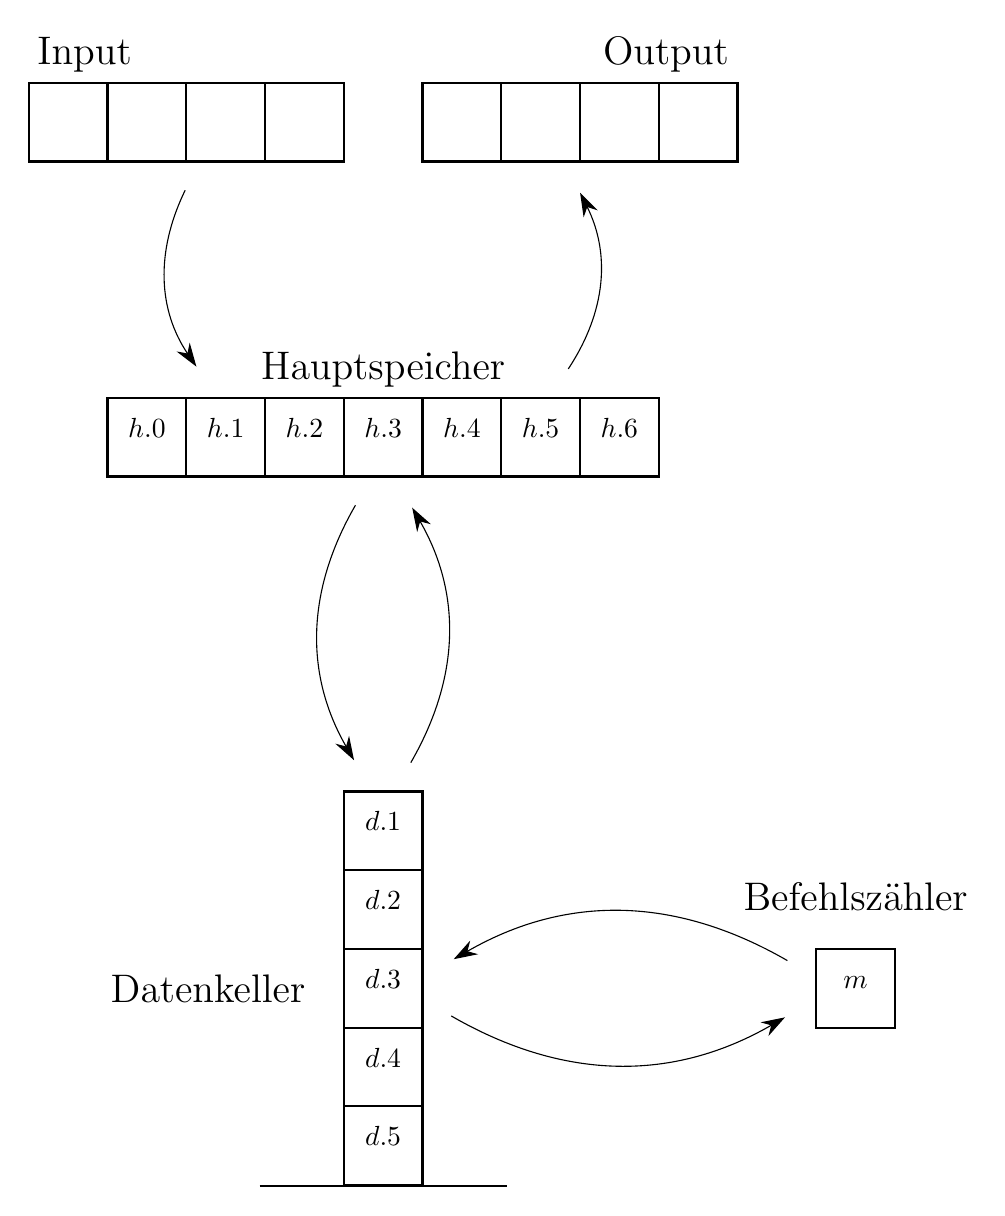
\begin{tikzpicture}
%		\foreach \i in {0,...,4} {
%			\draw[draw=black] (0,-\i) rectangle ++(3,-1) node[pos=.5] (h\i) {$h.\i$};
%			\draw[draw=black] (7,-\i) rectangle ++(3,-1) node[pos=.5] (d\i) {$d.\i$};
%		}
		
%		\node[below=of h4](HSText){Hauptspeicher};
%		\node[below=of d4](DKText){Datenkeller};
%		\node[above right=of h2](HS){};
%		\node[above left=of d2](DK){};
%		\node[below right=of h2](HS2){};
%		\node[below left=of d2](DK2){};
%		\draw[->] (HS) -- (DK);
%		\draw[->] (DK2) -- (HS2);
		
		\foreach \i in {0,1,2,3} {\\
			\node[fit={(\i,2) (\i+1,3)}, inner sep=0pt, draw, thick, align=center] (inp\i) {};
			\node[fit={(\i+5,2) (\i+5+1,3)}, inner sep=0pt, draw, thick, align=center] (out\i) {};
%			\draw[] (\i,2) rectangle ++(1,1) node[pos=.5] (inp\i) {};
%			\draw[] (\i+5,2) rectangle ++(1,1) node[pos=.5] (out\i) {};
		}
		
		\node[beschriftung, above=0em of inp0.north west, anchor=south west, align=left] (inpText){Input};
		\node[beschriftung, above=0em of out3.north east, anchor=south east, align=right](outText){Output};
	
	
		% HAUPTSPEICHER
		\foreach \i in {0,...,6} {
			\node[fit={(\i+1,-1) (\i+2,-2)}, inner sep=0pt, draw, thick, align=center] (h\i) {$h.\i$};
%			\draw[] (\i,-4) rectangle ++(1,1) node[pos=.5] (h\i) {$h.\i$};
		}
		\node[beschriftung, above=0em of h3](HSText){Hauptspeicher};
%				\draw[arrow,  bend angle=45, bend left] (HSText) -- (4.5,2);
		\draw[myarrow]     ([xshift= 1em, yshift=1em]h5.north) to[bend right] ([xshift= 0em, yshift=-1em]out2.south west);
		\draw[mybackarrow] ([xshift=-1em, yshift=1em]h1.north) to[bend left]  ([xshift= 0em, yshift=-1em]inp2.south west);
		
		
		% DATENKELLER
		\foreach \i in {1,...,5} {
			\node[fit={(4,-5-\i) (5,-6-\i)}, inner sep=0pt, draw, thick, align=center] (d\i) {$d.\i$};
%			\draw[red] (rect.east) to[out=0,in=-90] (rect.south);
%			\draw[] (5,-5 - \i) rectangle ++(-1,-1) node[pos=.5] (d\i) {$d.\i$};
		}
		\draw[thick] ([xshift=-3em]d5.south west) to ([xshift= 3em]d5.south east);
		\node[beschriftung, left=1em of d3, align=right, anchor=east](DKText){Datenkeller};
		
		\draw[myarrow]     ([xshift= 1em, yshift=1em]d1.north) to[bend right] ([xshift= 1em, yshift=-1em]h3.south);
		\draw[mybackarrow] ([xshift=-1em, yshift=1em]d1.north) to[bend left]  ([xshift=-1em, yshift=-1em]h3.south);
		
%		\node[fit={(5,-14) (4, -15)}, inner sep=0pt, draw, thick, align=center] (bz) {$m$};
%		\node[left=of bz](BZText){Befehlszähler};
%		
%		\draw[myarrow]     ([xshift= 1em, yshift=1em]bz.north) to[bend right] ([xshift= 1em, yshift=-1em]d5.south);
%		\draw[mybackarrow] ([xshift=-1em, yshift=1em]bz.north) to[bend left]  ([xshift=-1em, yshift=-1em]d5.south);

		\node[fit={(10,-8) (11, -9)}, inner sep=0pt, draw, thick, align=center] (bz) {$m$};
		\node[beschriftung, above=1em of bz](BZText){Befehlszähler};
		
		\draw[myarrow]     ([xshift=-1em, yshift= 1em]bz.west) to[bend right] ([xshift= 1em, yshift= 1em]d3.east);
		\draw[mybackarrow] ([xshift=-1em, yshift=-1em]bz.west) to[bend left]  ([xshift= 1em, yshift=-1em]d3.east);
		
	\end{tikzpicture}
\end{document}